\newprob{1716021004}
{
    % aristo q7
    光從相同的未知介質通過進入每個液體1、2、3和4時的入射角和折射角如下所示。哪個液體$(1,2,3,4)$具有最高的折射率?
    % \\The angles of incidence and refraction when light passes from an unknown medium into each liquid 1, 2, 3 and 4 are shown below. Which liquid has the highest refractive index?
    \begin{tasks}(2)
        \task \topalign{\par\centering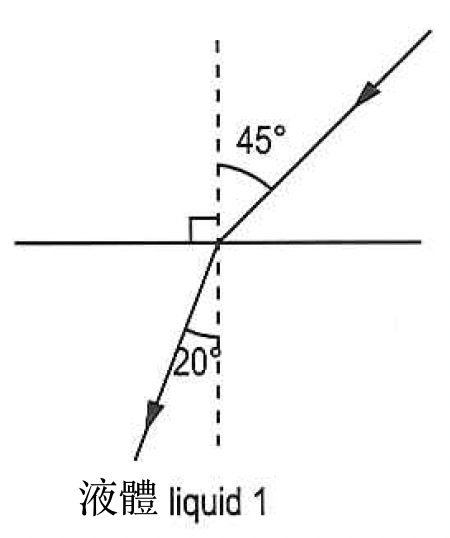
\includegraphics[width=.28\textwidth]{./img/ch2_refraction_mc_2024-05-18-16-32-14.png}\par}
        \task \topalign{\par\centering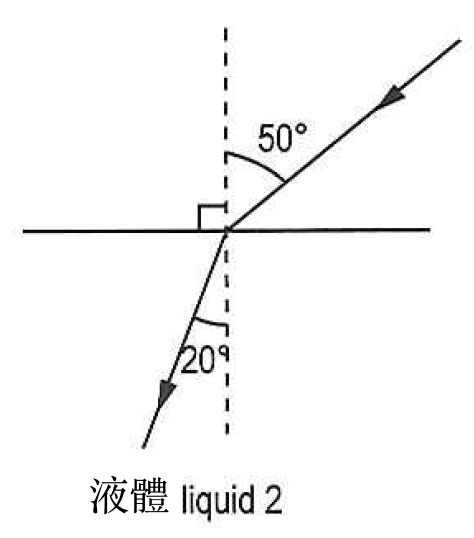
\includegraphics[width=.3\textwidth]{./img/ch2_refraction_mc_2024-05-18-16-32-44.png}\par}
        \task \topalign{\par\centering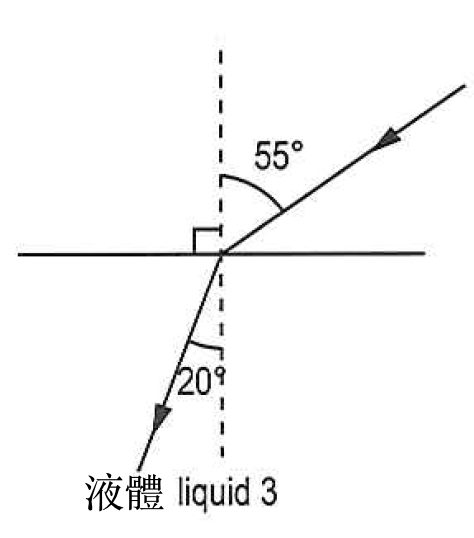
\includegraphics[width=.3\textwidth]{./img/ch2_refraction_mc_2024-05-18-16-33-17.png}\par}
        \task \topalign{\par\centering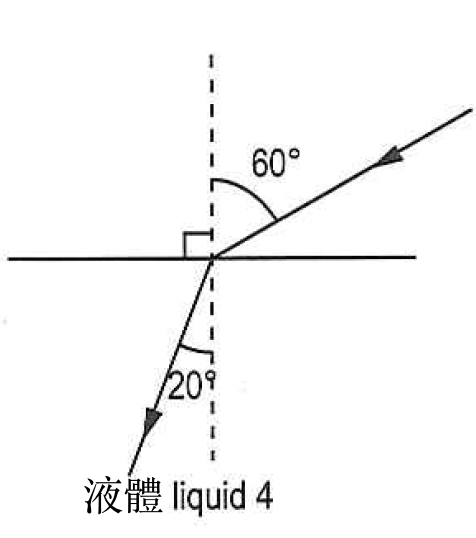
\includegraphics[width=.3\textwidth]{./img/ch2_refraction_mc_2024-05-18-16-34-00.png}\par}
    \end{tasks}

    \itsquestionfalse
}{D}


\newprob{1716021451}
{
    % aristo q12
    \uplevel{\textbf{Question 2 - Question 4}}
    一束光線PQ從空氣中入射到一個矩形塊WXYZ的面WZ。光線在塊內彎曲,沿著RS方向出射矩形塊體,如下圖所示。
    \par{\par\centering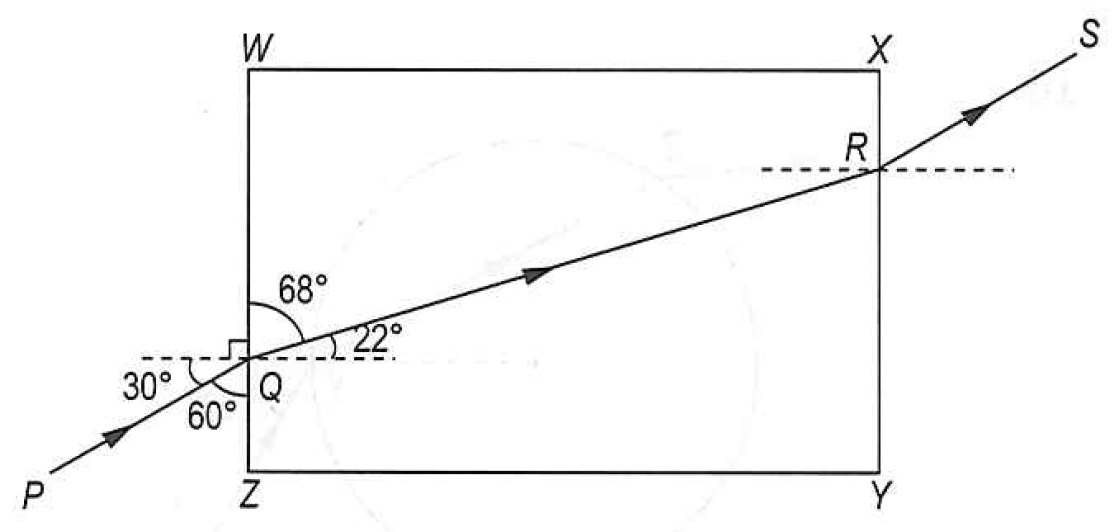
\includegraphics[width=.4\textwidth]{./img/ch2_refraction_mc_2024-05-18-16-38-40.png}\par}
    % A light ray PQ strikes the face WZ of a rectangular block WXYZ from air. The light ray bends along the direction QR inside the block and emerges the block in the direction Rs as shown in the diagram below.
}{}

\newprob{1716021541}
{
    矩形塊WXYZ的材料的折射率是多少?
    % What is the refractive index of the material of the rectangular block WXYZ?
    \begin{tasks}
        \task 0.54
        \task 0.93
        \task 1.33
        \task 2.31
    \end{tasks}

}{C}

\newprob{1716021591}
{
    在矩形塊的XY表面上,光線在R處的入射角是多少?
    % What is the angle of incidence of the light ray at R on the surface XY of the rectangular block?
    \begin{tasks}
        \task \dg{22}
        \task \dg{30}
        \task \dg{60}
        \task \dg{68}
    \end{tasks}

}{A}

\newprob{1716021640}
{
    如果一束光線不是從空氣中射向Q,而是從空氣中射向R,並沿著方向RQ折射進入矩形塊,則在R處的入射角是多少?
    % If a light ray instead of hitting Q from air, it hits the block at R from air and refracts into the rectangular block along the direction RQ, what is the angle of incidence at R?
    \begin{tasks}
        \task \dg{22}
        \task \dg{30}
        \task \dg{60}
        \task \dg{68}
    \end{tasks}
}{B}

\newprob{1716021801}
{
    % q18
    一束光線通過三種介質,如下圖所示。
    % A ray of light passes through three media as shown below.
    \par{\par\centering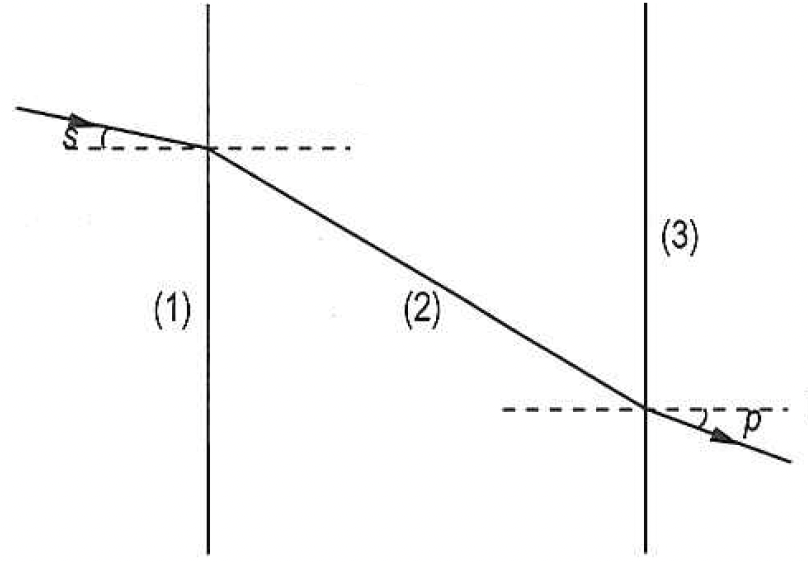
\includegraphics[width=.4\textwidth]{./img/ch2_refraction_mc_2024-05-18-16-43-24.png}\par}
    $p$ > $s$,以下哪個是三種介質的可能組合? $\;$ (已知:$n_{\textrm{玻璃}}=1.52$, $n_{\textrm{水}}=1.33$)
    % Given that p > s. Which of the following is a possible combination of the three media?
    \begin{tasks}
        \task [] (1)\tab (2)\tab (3)
        \task 空氣 \tab 玻璃 \tab 水
        \task 玻璃 \tab 水 \tab 空氣
        \task 玻璃 \tab 空氣 \tab 水
        \task 水 \tab 空氣  \tab 玻璃
    \end{tasks}
}{C}



\newprob{mc1}{
    一束由紅光和紫光組成的光線,射向矩形玻璃 塊。以下哪圖最能表示,光線通過玻璃塊的路徑?
    % \\A ray consists of red and violet light, Which of the following best shows the paths of the ray through n rectangular block?
    \begin{tasks}(2)

        \task
        \topalign{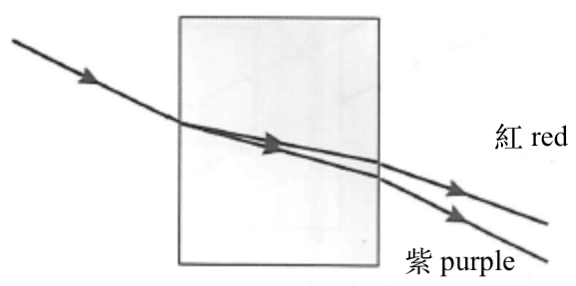
\includegraphics[width=0.8\linewidth]{d21d1d017.png}}
        \task
        \topalign{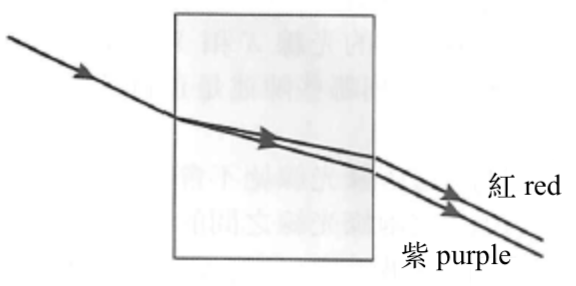
\includegraphics[width=0.8\linewidth]{xn98eu9e29n332f.png}}
        \task
        \topalign{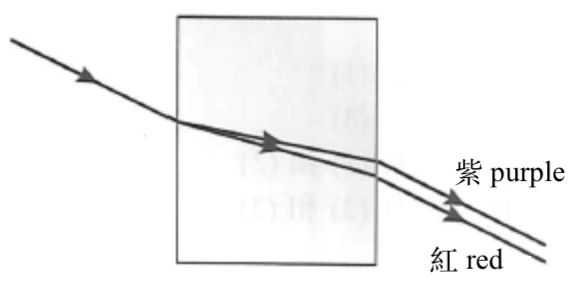
\includegraphics[width=0.8\linewidth]{dn0xu9dn23.png}}
        \task
        \topalign{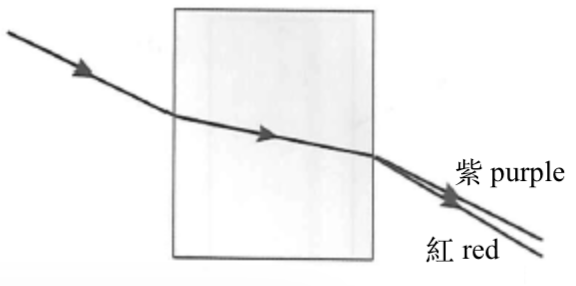
\includegraphics[width=0.8\linewidth]{x8un892.png}}

    \end{tasks}
}{C}

\newprob{mc2}{
光線X從空氣沿法線射向玻璃三稜鏡 ABC,如上 圖所示。若整個裝置浸在水中,將會出現什麼結果?
% \\A ray of light X travels in air and strikes a glass prism ABC normally as shown above. What happens if the setup is immersed in water?
{\par\centering
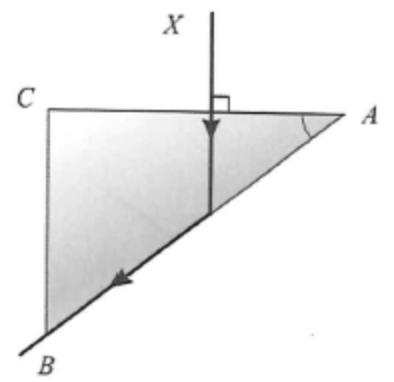
\includegraphics[width=0.25\linewidth]{xeu98neu32e3.png}\par}
\begin{tasks}
    \task 光線將在棱鏡內發生全內反射,然後 從 BC上某點離開。
    % \\The ray will undergo total internal reflection inside the prism and then emerge from a point on BC.
    \task 光線將直線穿過 AB 而不會改變方向。
    % \\The ray will pass straight through AB without change in direction.
    \task 光線將通過 AB 並偏折,在左邊射出。
    % \\The ray will pass through AB and bend to the left side.
    \task 光線將通過 AB並偏折,在右邊射出。
    % \\The ray will pass through AB and bend to the right side.
\end{tasks}
}{C}

\newprob{mc3}{
    \topalignc{\par\centering
        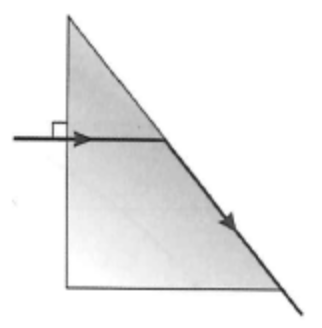
\includegraphics[width=0.25\linewidth]{d89q98ndwq.png}\par}\par
    一束窄的紅光,沿法線射向玻璃三棱鏡,然後 離開,如上圖所示。若以紫光取代紅光,下列 哪圖最能代表光束新的路徑?
    % \\A narrow beam of red light strikes a triangular glass prism normally and emerges as shown above. If the beam is replaced by violet light, which of the following diagrams best represents the path of light?
    \begin{tasks}(2)
        \task
        \topalign{\par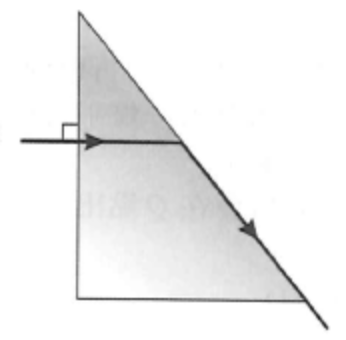
\includegraphics[width=0.6\linewidth]{und89wqudage.png}\par}


        \task
        \topalign{\par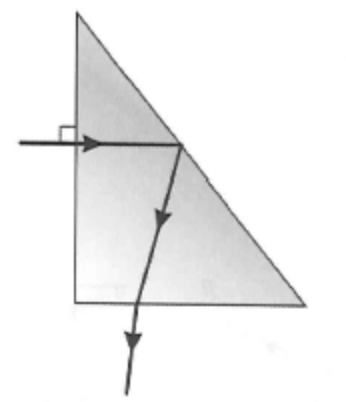
\includegraphics[width=0.6\linewidth]{djioqwge.png}\par}


        \task
        \topalign{\par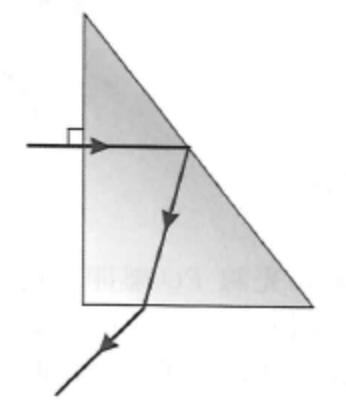
\includegraphics[width=0.6\linewidth]{diqwdoiqw2.png}\par}


        \task
        \topalign{\par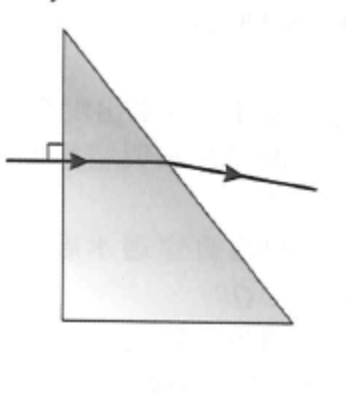
\includegraphics[width=0.6\linewidth]{dwq1d1dcddd13.png}\par}


    \end{tasks}
}{C}
\newprob{mc4}{
    \topalignc{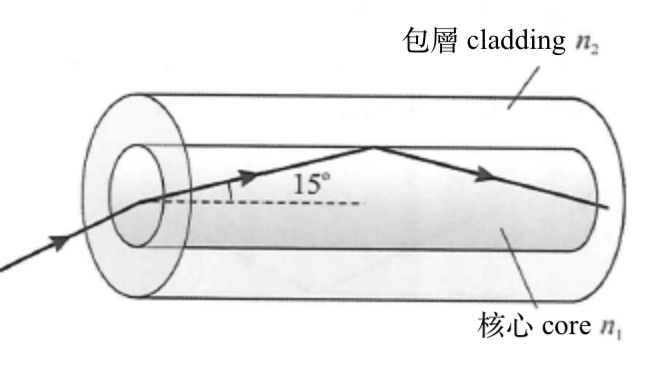
\includegraphics[width=0.5\linewidth]{d2nuc9u8293uc2nr23.png}}
    光導纖維的玻璃核芯(折射率 $n_1$)以包層(折 射率 $n_2$)包裹著。上圖顯示一條光線從空氣進 入玻璃核心,並經過一次全內反射。下列哪些 陳述是正確的?
    % \\The glass core (refractive index $n_1$) of an optical fibre is surrounding by a cladding (refractive index $n_2$). The diagram shows how a ray of light enters into the glass core and then undergoes total internal reflection. Which of the following statements is/are true?
    \begin{statements}
        \task 玻璃核心和包層之間的臨界角大於 \dg{75}。
        % \\The critical angle between the glass core and the cladding is greater than \dg{75}.
        \task $n_1>n_2$
        \task $n_1>\dfrac{1}{\sin 75^\circ}$
    \end{statements}
    \begin{tasks}
        \task 只有(1)
        %  \tab\tab (1) only
        \task 只有(3)
        % \tab\tab (3) only
        \task 只有(1)和(2)
        % \tab\tab (1) and (2) only
        \task 只有(2)和(3)
        % \tab\tab (2) and (3) only
    \end{tasks}
}{D}
\newprob{mc5}{
    \topalignc{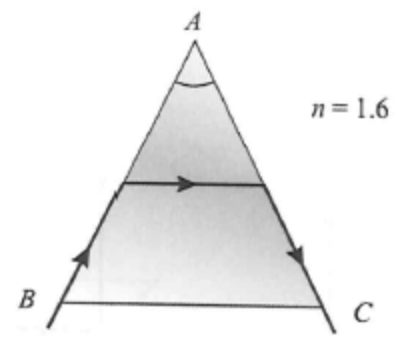
\includegraphics[width=0.3\linewidth]{x98nu823.png}}\par
    三棱鏡 ABC 所用材料的折射率為1.6。一條 光線沿棱鏡的一面入射,並沿棱鏡的另一面離 開,如上圖所示。棱鏡上的角A 是多少?
    % \\A triangular prism ABC is made of material of refractive index 1.6. A ray of light at glancing incidence leaves the prism also at glancing angle as shown. What is the angle A of the prism?
    \begin{tasks}
        \task \dg{39}
        \task \dg{56}
        \task \dg{65}
        \task \dg{77}
    \end{tasks}

}{D}
\newprob{mc6}{
    \topalignc{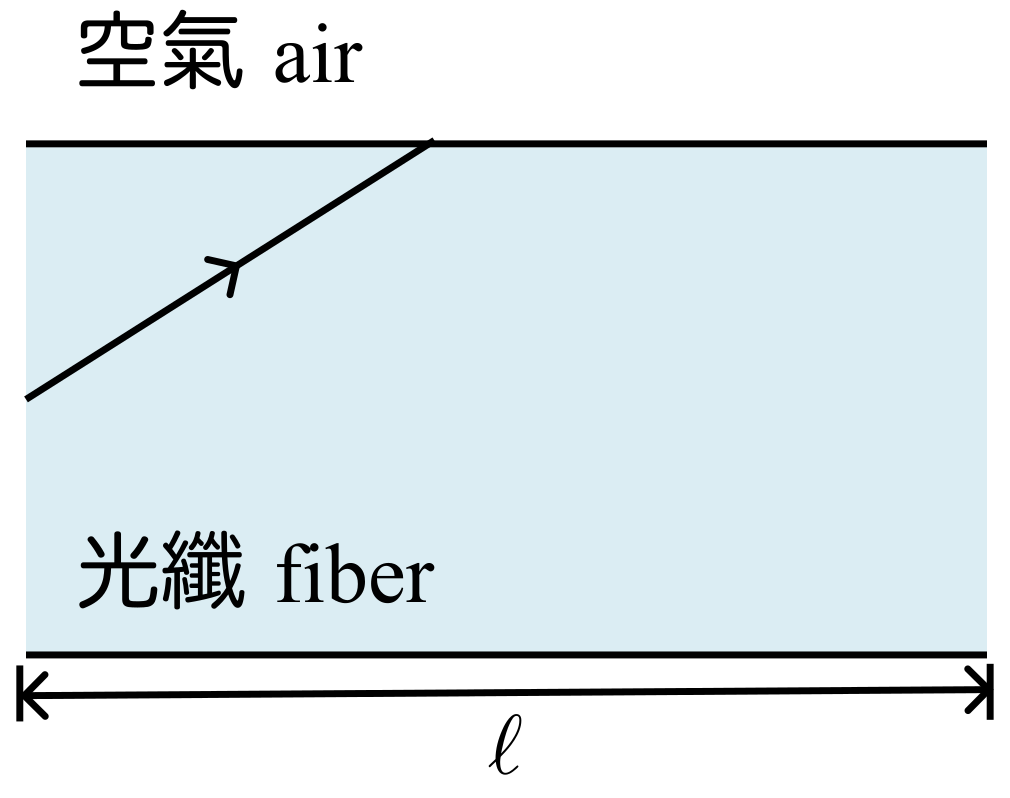
\includegraphics[width=0.3\linewidth]{dqwijqwoe.png}}
    一條光線沿筆直的光纖傳播。已知光纖長度為 $\ell$,折射率為 $n$。光線從光纖一端傳播至另一端 的最短及最長時間分別是多少?設$c$為光在真空 中的速率。
    % \\A light ray travels in a straight fibre of refractive index $n$ and length $\ell$. What are the min. and max. time required for the light to travel from one end of the fibre to the other end without any light leak? ($c$: speed of light in vacuum)
    \begin{tasks}
        \task [] 最短時間\tab\tab 最長時間
        \task $\dfrac{\ell}{nc}$\tab\tab $\dfrac{n\ell}{c}$
        \task $\dfrac{\ell}{nc}$\tab\tab $\dfrac{n^2\ell}{c}$
        \task $\dfrac{n\ell}{c}$\tab\tab $\dfrac{n^2\ell}{c}$
        \task $\dfrac{n\ell}{c}$\tab\tab $\dfrac{n^4\ell}{c}$
    \end{tasks}
}{C}
\newprob{mc7}{
    \topalignc{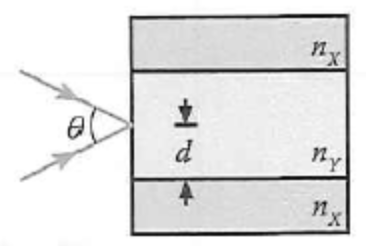
\includegraphics[width=0.25\linewidth]{d9i09n293d.png}}\medskip
    \par 一條纖維由包層(折射率 $n_X$)及核心(折射率 $n_Y$)組 成。光線在圖中所示、頂 角為$\theta$的圓錐範圍內射入 纖維,便可透過全內反射 傳播至遠處。核心的半徑 為$d$,如圖。
    % \\A fibre is made of a core (refractive index = $n_Y$) embedded in a cladding (refractive index = $n_X$). Its core has a radius $d$. Light rays within a cone of vertex angle $\theta$ at the central axis of the fibre can be guided through the fibre by total internal reflection.
    \par 要增加$\theta$的值,可以
    % \\The angle $\theta$ can be increased by
    \begin{statements}
        \task 減少$d$的值。
        % \\reducing d.
        \task 減少$n_X$的值。
        % \\reducing $n_X$
        \task 減少$n_Y$的值。
        % \\reducing $n_Y$
    \end{statements}
    \begin{tasks}
        \task 只有(2)
        % \tab\tab (2) only
        \task 只有(3)
        % \tab\tab (3) only
        \task 只有(1)和(2)
        % \tab\tab (1) and (2) only
        \task 只有(1)和(3)
        % \tab\tab (1) and (3) only
    \end{tasks}
}{A}

\newprob{mc8}{
一束光線投射至一塊長方形玻璃磚。玻璃磚闊度 為$w$,折射率為$n$。光線以角度$\theta$進入玻璃磚 後,產生旁向位移$d$,如圖。下列哪情況能增加 $d$的值?
% \\A rectangular glass block has a width $w$ and a refractive index $n$. When a light ray strikes it at an angle $\theta$ as shown, the emergent ray is laterally displaced by a distance $d$. In which of the following situations will the value of $d$ increase?
{\par\centering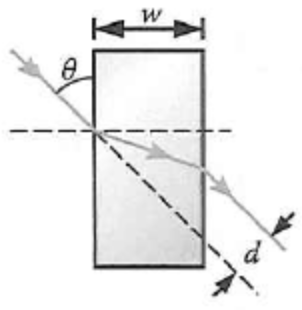
\includegraphics[width=0.22\linewidth]{8x9nu23.png}\par}
\begin{statements}
    \task 增加$n$ 的值
    % \\$n$ increases
    \task 增加$\theta$ 的值
    % \\$\theta$ increases
    \task 增加$w$ 的值
    % \\$w$ increases
\end{statements}
\begin{tasks}
    \task 只有(1)和(2)
    % \tab\tab (1) and (2) only
    \task 只有(1)和(3)
    % \tab\tab (1) and (3) only
    \task 只有(2)和(3)
    % \tab\tab (2) and (3) only
    \task (1), (2) 和 (3)
    % \tab\tab (1), (2) and (3)
\end{tasks}

}{D}